%------------------------------------------------------------------------------%
%                                   cholesky                                   %
%------------------------------------------------------------------------------%

\section{Cholesky}

\gls{fds}'s simulation requires to solve equations. For this they are able to
use the Cholesky algorithm, however, their current implementation is not fast
enough. In this section, we will start by presenting the algorithm. Then we
will explain the implementation with \gls{hh} before presenting the results. For
the measures, our implementation will be compared to the openblas's one as it is
one of the fastest currently available.

\subsection{The algorithm}
\label{sec:choalgo}

The Cholesky algorithm is used to solve systems of linear equations of the form
$Ax = y$ where $A \in M_{n,n}(\mathrm{R})$ is symmetric and positive-definite
\cite{choleskywiki}. The principle is to decompose the matrix $A$ into a matrix
$L$ such as $A = LL^{T}$ where $L \in M_{n,n}(\mathrm{R})$ is a lower triangular
matrix. Then, we can solve the two sub-problems: $Lx' = y$ and $L^{T}x = x'$.

There are several ways to implement this algorithm. Here, we are going to
implement the block version since it is the most adapted to parallel computing.
Indeed, one most important notions of \gls{hpc} is the optimization of the CPU
cache usage. To do this, we will decompose our matrix into smaller blocks that
can be entirely loaded into the cache in order for the CPU not to access the
RAM.

The version of the algorithm that we will use is explained by
\cite{choleskyblock}. This algorithm is done in three steps. First, let's
consider the matrix $A$ visible on the figure \ref{fig:chodeca}. On this figure,
$D$ is a diagonal block, $C$ is a column (composed of multiple blocks) and $A'$
is a sub-matrix.

% [Cholesky decomposition] {{{
\begin{figure}[!ht]
  \begin{center}
    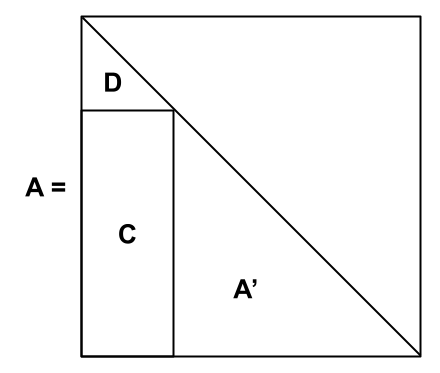
\includegraphics[scale=0.4]{img/cho-img/cho_block_dec_A.png}
    \caption{Cholesky decomposition: matrix A}
    \label{fig:chodeca}
  \end{center}
\end{figure}
%}}}

The first step of the algorithm is to treat the diagonal element $D$. To do
this, we use the sequential version of the algorithm. It will be fast enough
considering the size of the block. The second step is to update the elements on
the column beneath the diagonal block. To do this, we solve the system $C_{new}
= C(D^{T})^{-1}$. Once it is done, we have computed the first column of the
result matrix $L$. The last step consists of updating the rest of the matrix $A$
by doing $A' = A' - CC^{T}$.

Once we have obtained the matrix $L$, we can proceed to the solving part to find
the solutions of the system. It can be decomposed in two steps: first, we solve
the equation with the diagonal block, then we update the rest of the matrix and
the result vector using the partial solution (we remove the variables from the
equation). We repeat these steps for each diagonal blocks to solve a
sub-problem. The solver must be used twice to solve the two sub-problems  $Lx' =
y$ and $L^{T}x = x'$.

\subsection{Implementation}

The implementation of the algorithm has been done in two parts. The
decomposition as been done first, and once it was fully functional, the solver
part has been added. This choice has been made because the decomposition is the
most critical piece of the algorithm. It was important to compare our version
with the openblas's one before implementing the solver.

The first implementation of the decomposition consisted of the creation of a
graph that followed the steps describe in the section \ref{sec:choalgo}
similarly to openblas. This graph is visible on the figure \ref{fig:chograph}.

% [Cholesky decomposition graph] {{{
\begin{figure}[!ht]
  \begin{center}
    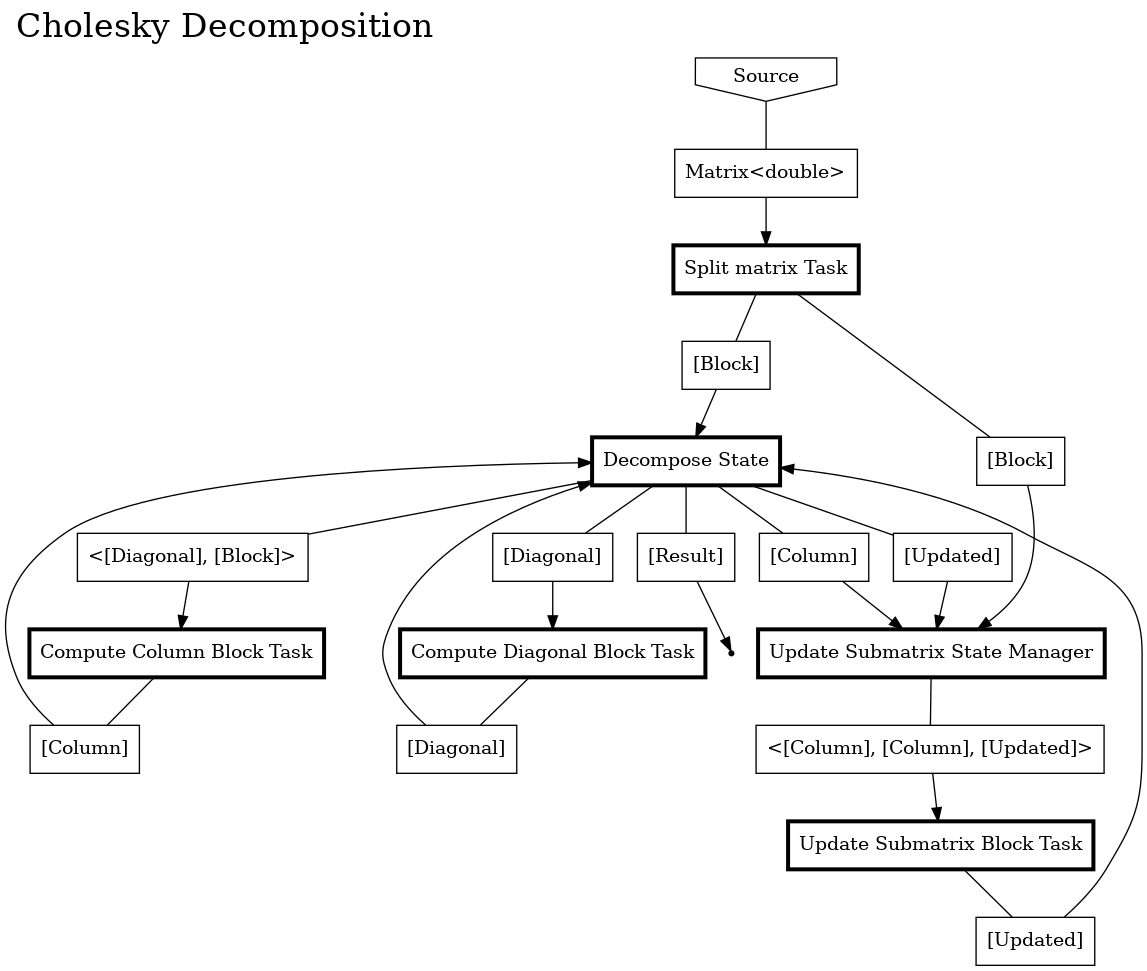
\includegraphics[scale=0.3]{img/cho-img/decompose_graph.png}
    \caption{Cholesky decomposition graph}
    \label{fig:chograph}
  \end{center}
\end{figure}
%}}}

On this diagram, the tasks and the states are represented by the bold rectangles
and the data by the regular rectangles. There are two kinds of datas that flow
into this graph. The first kind is the \texttt{Matrix} that is the input of the
graph and the second kind is the matrix blocks represented by the block's
identifier between \texttt{'[]'}. The matrix is given to the \texttt{Split Task}
that generates the blocks. The blocks have identifiers, which define their
types. These identifiers are used to send the right blocks to the right task (or
state). For instance, when the \texttt{Decompose State} sends a
\texttt{Diagonal} block, it is transferd to the \texttt{Compute Diagonal Block
Task}. We might see the execution of this graph as follows:

\begin{enumerate}
  \item Split the matrix into blocks (\texttt{Split Matrix Task}).
  \item Compute the diagonal element \textbf{C} (\texttt{Compute Diagonal Block Task}).
  \item Compute the elements on the column \textbf{D} (\texttt{Compute Column Block Task}).
  \item Update the sub-matrix \textbf{A'} (\texttt{Update State / Task}).
  \item Restart from 2 with the blocks of \textbf{A'} (and send the result
    blocks).
\end{enumerate}

This first solution was too slow since we were executing the three steps
sequentially (this is also what is done in openblas). By doing so, we were
loosing a lot of parallelism. For instance, the computation of the diagonal
elements could be done with only one thread and all the other threads had to
wait. To optimize the algorithm, we wanted to keep the threads as busy as
possible and the solution for this was to rely on early computation by
processing the blocks as soon as they are ready. For instance, we can start
solving the next diagonal element before all the blocks of the sub-matrix $A'$
are updated. We can do the same thing with the column blocks.

To make the early computation possible, the block's data structure has been
changed. A \texttt{rank} attribute has been added to keep track of the
modifications on the blocks. Each time a block is updated, its rank is
increased. When the rank of a block is equal to its column number, it is ready
to be processed, and it is processed when its rank is superior to its column
number. The states use pending lists to store indices of blocks that should be
processed, and iterate on these lists to launch the computation of all ready
blocks. The graph concerves the same structure, but the operations in the state
have been drastically changed.

In this second version, there are a lot of verifications to make, using the rank
in the states. Furthermore, both of the states have a vector of block pointers
that are shared between them to make sure that when the \textit{decompose state}
changes a rank, the \textit{update state} can be aware of the modification
directly, without any notification. This improves the performances but adds more
complexity in the states.

Eventually, we managed to have good performances with this second version since
openblas does not make any early computation. We will describe our results in
the section \ref{sec:chores}.

For the solver, we have a second graph that we use twice to solve the two
sub-system of the matrix. The graph can be seen on the figure
\ref{fig:solvergraph}.

% [Solver graph] {{{
\begin{figure}[!ht]
  \begin{center}
    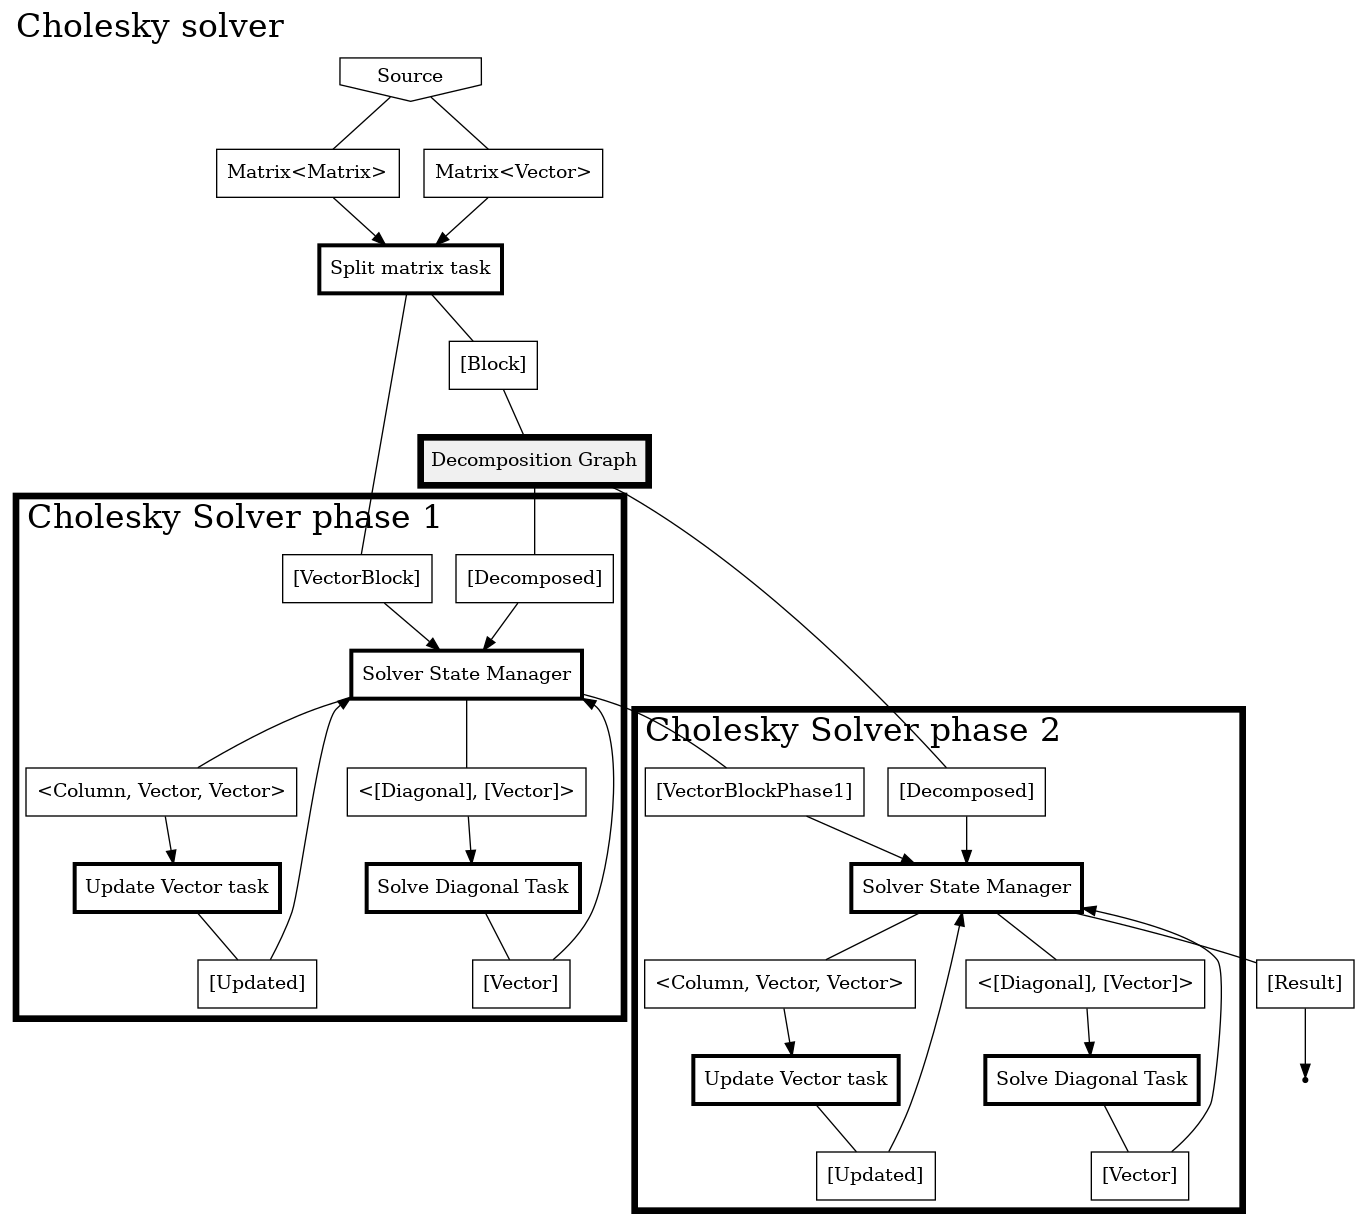
\includegraphics[scale=0.2]{img/cho-img/solver_graph.png}
    \caption{Solver graph}
    \label{fig:solvergraph}
  \end{center}
\end{figure}
%}}}
%todo: explain the solver graph

Here, we can see that there are two subgraphs for the solving part. These two
graphs solve the two sub-problems that we described earlier. The fist solver is
directly connected to the decomposition's graph, and it receives the decomposed
block. Both of the solver graphs are connected to the split task, and they
receive the splited vector blocks.

In this graph we use the same matrix blocks as in the decomposition graph, so we
can start the solving part directly when the decomposition graph outputs the
first result block. The hole principle of \gls{hh} is to allow the creation of
pipelines in which the datas flow continuously, so we avoid having unecessary
barriers\footnote{Points in the program where we have to wait for the
termination of task to start the next one} in the process. Here, we do not have
to finish the decomposition entirely to start solving the blocks. This helps
keeping as much parallelism as possible and always use the biggest amount of the
computer's resources. In other words, if we represented the computation time
between the logical cores in a Gantt diagram, we would like to optimize the
overlap between tasks and have as little gaps as possible (the cores should not
be in a wait state for too long, at all ideally).

\clearpage{}
\subsection{The results}
\label{sec:chores}

Now that we have explained the algorithm and its implementation, we will analyse
the results of the measures on the decomposition algorithm that have been done
using the openblas's implementation hand the \gls{hh}'s one. Two sets of
measures have been made on cluster node with 192 CPU cores. For the first set,
the problem size was 40000 and the program has been run with a maximum number of
threads of 256. For the second set, we used a 100000 matrix and a maximum number
threads of 384 (all the cores). On each problem, we were measuring the
computation times of the two algorithm for different number of threads (from 1
to the maximum) in order to see the relative speedup. For \gls{hh}, the number
of threads was changed only for the most critical task (the update task). It was
fixed to the optimal numbers for the other tasks (these numbers were found by
doing first tests measures beforehand).\\

First, we can analyse the measures made on the 40000 matrix. The figure
\ref{fig:40000graph} is the graph that is generated at the end of the program
using \gls{hh}'s profiling tool. Here we can see that the bottleneck of the
program is effectively the update task as we have explained before. We can see
as well that only one thread was allocated to the diagonal task and 12 were
allocated to the column task. The diagonal does not require more that one thread
since it never have more than one block (this is shown by the maximum queue size
\texttt{MQS} on the rectangle before the task). For the column task, we can see
that it is relatively slow (if we look at the color). We could put more threads
on it, but we have to make sure that we keep enough resources for the update
task.

% [Hedgehog graph for the 40000 matrix] {{{
\begin{figure}[!ht]
  \begin{center}
    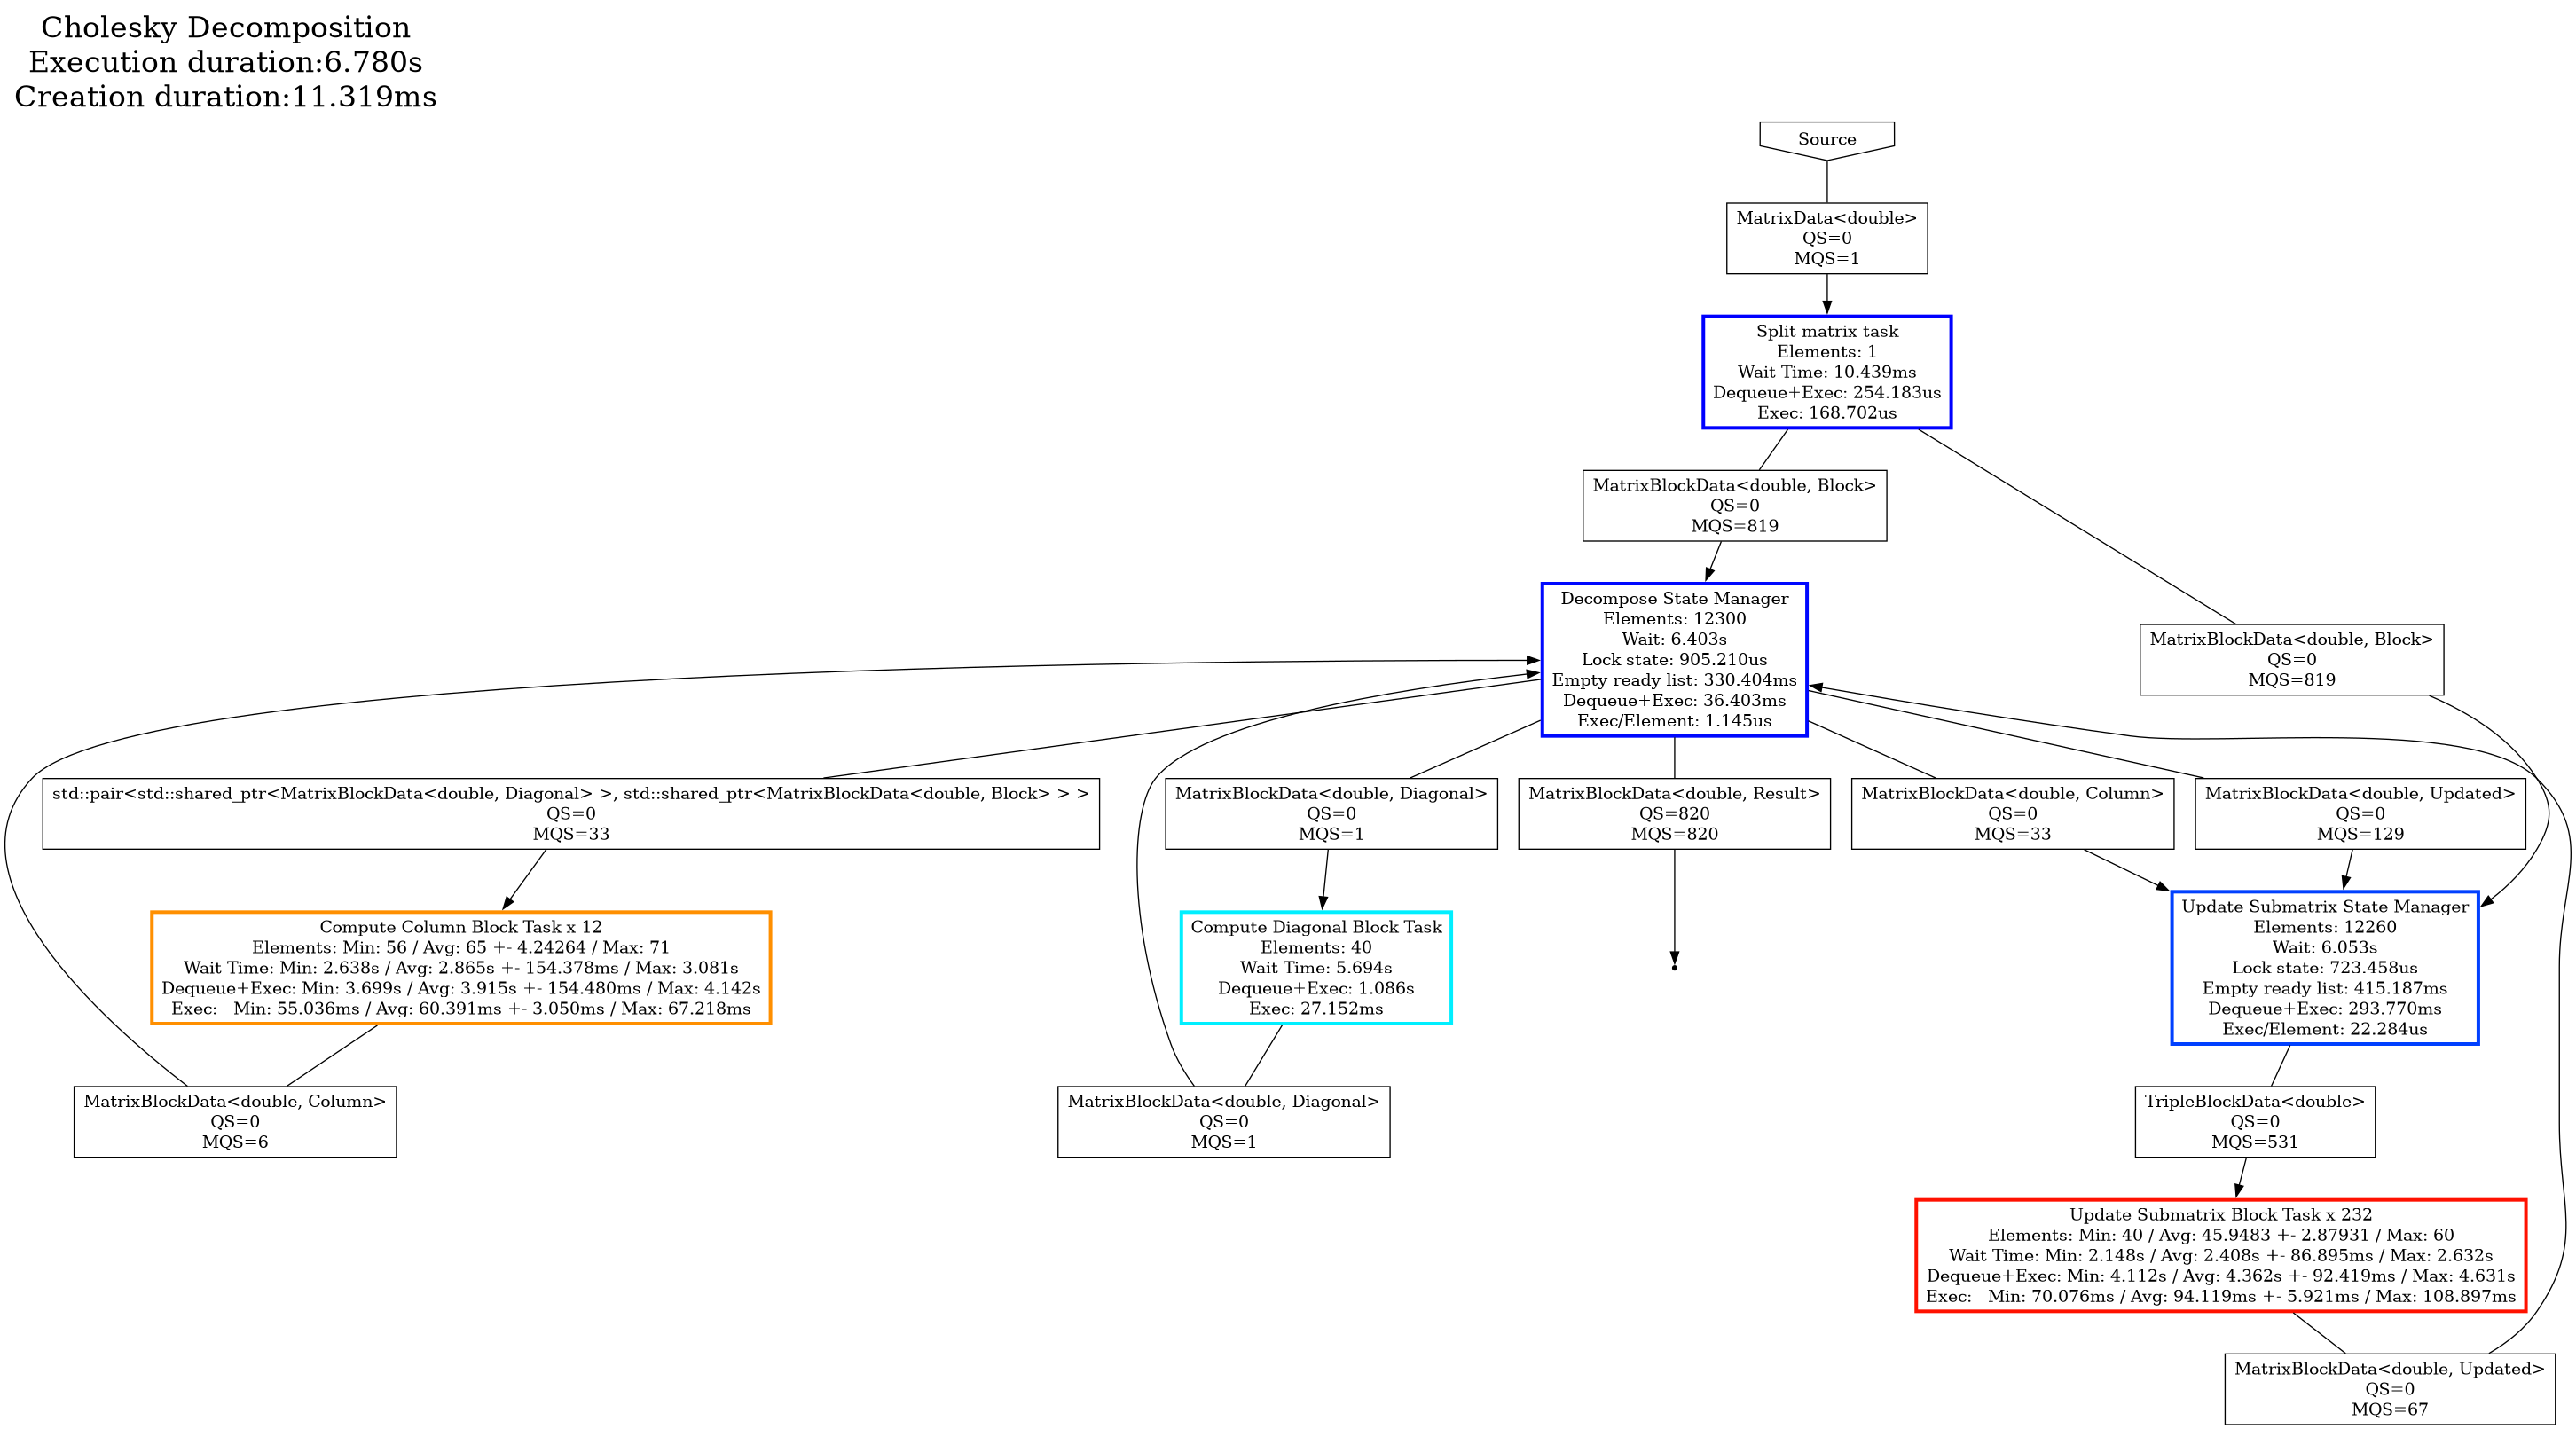
\includegraphics[scale=0.15]{img/cho-img/40000.png}
    \caption{Hedgehog graph for the 40000 matrix}
    \label{fig:40000graph}
  \end{center}
\end{figure}
%}}}

On the figures \ref{fig:time40000} and \ref{fig:speedups40000} we see the
computation times of the two implementations and the speedup of the \gls{hh}'s
version compared to the openblas's one for the 40000 matrix. Here, we can
observe a very interesting behavior of the openblas program. As we increase the
number threads, the \gls{hh} program keeps scaling but the openblas's one become
unstable around a hundred threads. A possible explanation for this is that
openblas is optimized for non-hyper-threaded configurations. For these measures,
we had allocated 256 threads on the cluster which means that we could have used
1 thread per core till more than 128 threads was allocated to the program. This
number is quite close to the point where we start to see instability on the
openblas's measures.

\begin{figure}[!htb]
  \begin{minipage}{0.48\linewidth}
    \centering
    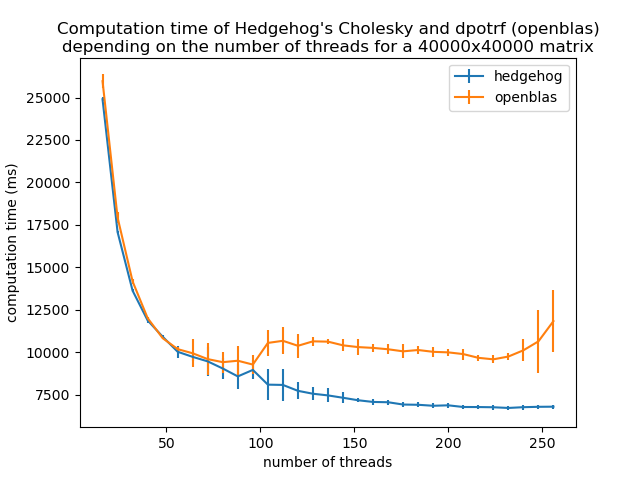
\includegraphics[scale=0.5]{img/cho-img/times-40000.png}
    \caption{Computation times for a 40000 matrix}
    \label{fig:time40000}
  \end{minipage}\hfill
  \begin{minipage}{0.48\linewidth}
    \centering
    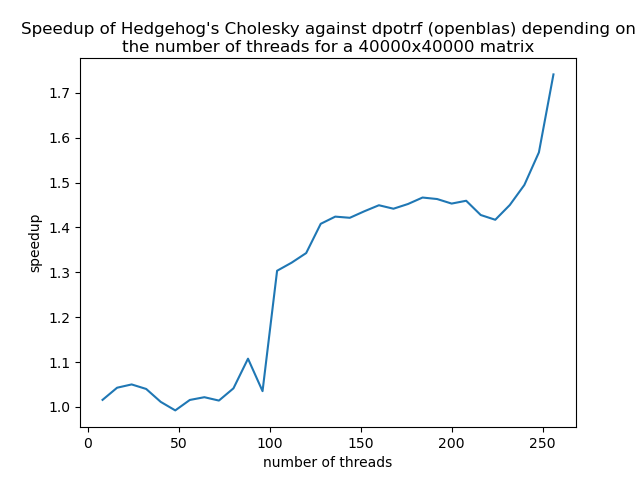
\includegraphics[scale=0.5]{img/cho-img/speedup-40000.png}
    \caption{Speedups for a 40000 matrix (hedgehog / openblas)}
    \label{fig:speedups40000}
  \end{minipage}
\end{figure}

The figure \ref{fig:relativespeedup40000} shows the relative speedup for each
program ($\frac{time_{one_thread}}{time_{n_thread}}$). As we can see, we do not
have a very big speedup for both of the programs. This can be explained by the
fact the current problem is too small, so we do not exploit the resources as
well as we should. For this reason, we have made more measures with a bigger
problem.

% [Relative speedups for a 40000 matrix] {{{
\begin{figure}[!ht]
  \begin{center}
    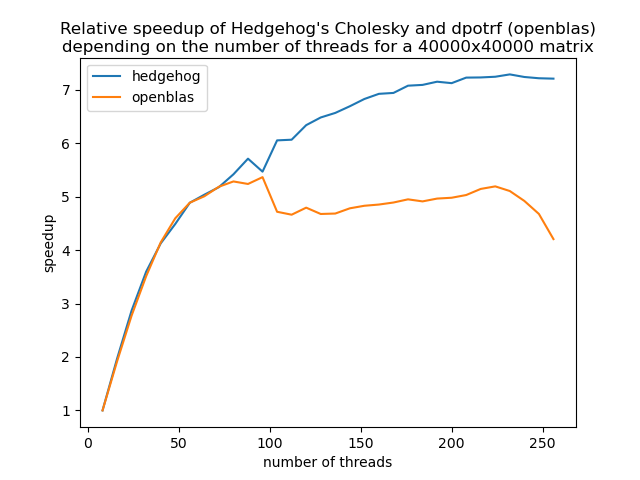
\includegraphics[scale=0.8]{img/cho-img/relative-speedup-40000.png}
    \caption{Relative speedups for a 40000 matrix}
    \label{fig:relativespeedup40000}
  \end{center}
\end{figure}
%}}}

The second set of measures was using a 100000 by 100000 matrix, and we went up to
384 threads. On the figure \ref{fig:time100000} and \ref{fig:speedups100000} we
can see the computation times of the two implementations as well as the speedup
of \gls{hh} against openblas as we have seen previously. These two plots shows
similar results than the previous ones.

\begin{figure}[!htb]
  \begin{minipage}{0.48\linewidth}
    \centering
    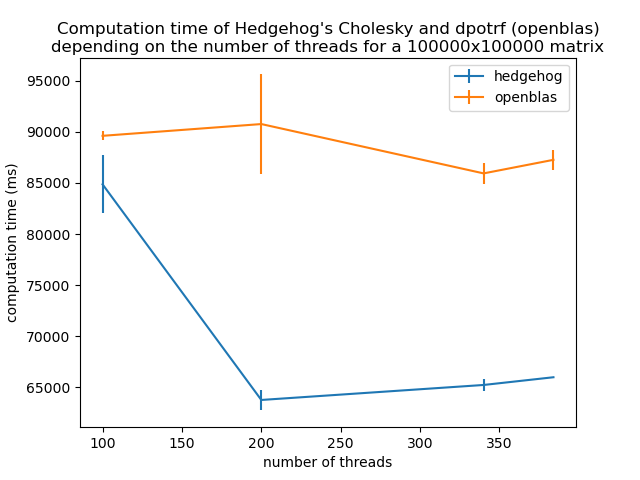
\includegraphics[scale=0.5]{img/cho-img/times-100000.png}
    \caption{Computation times for a 100000 matrix}
    \label{fig:time100000}
  \end{minipage}\hfill
  \begin{minipage}{0.48\linewidth}
    \centering
    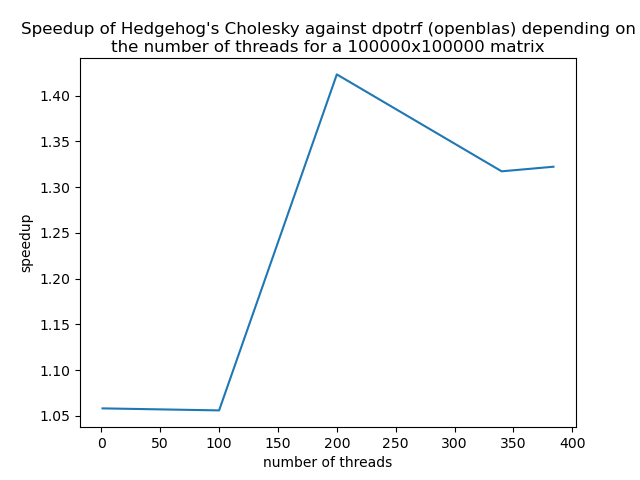
\includegraphics[scale=0.5]{img/cho-img/speedup-100000.png}
    \caption{Speedups for a 100000 matrix (hedgehog / openblas)}
    \label{fig:speedups100000}
  \end{minipage}
\end{figure}

On the figure \ref{fig:relativespeedup100000} we can see that we have a way
better relative speedup for the two algorithms. This means that the resources
are better exploited with a bigger problem.

% [Relative speedups for a 100000 matrix] {{{
\begin{figure}[!ht]
  \begin{center}
    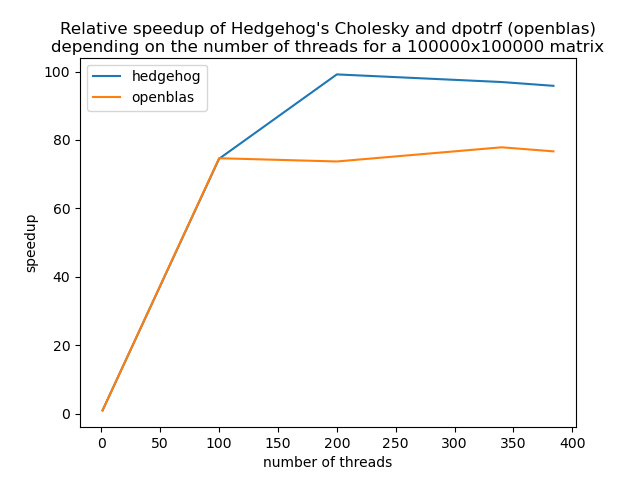
\includegraphics[scale=0.8]{img/cho-img/relative-speedup-100000.png}
    \caption{Relative speedups for a 100000 matrix}
    \label{fig:relativespeedup100000}
  \end{center}
\end{figure}
%}}}

Eventually, we managed to have better performances than openblas by doing more
early computation. Furthermore, the program is still readable and easy to
understand. This demonstrates how good is the data-flow graph approach is in
parallel computing as well as the power of the \gls{hh} library.
